\subsection{采样与采样定理}

研究连续时间信号与离散时间信号之间的关系时,我们最关心什么?
\begin{itemize}
    \item 在什么条件下,一个连续时间信号可以用它的离散时间样本
        来代替而不致丢失原有的信息?
    \item 如何从连续时间信号的离散时间样本不失真地
        恢复成原来的连续时间信号?
\end{itemize}

\subsubsection{采样的数学模型}

\begin{property}
    在没有任何条件限制的情况下,从连续时间信号采样
    所得到的样本序列\bd{不能}唯一地代表原来的连续时间信号。
\end{property}

\begin{example}
    如图 \ref{fig:counterexample-sampling} 所示,
    三个信号在 $t = -3T, -2T, -T, 0, T, 2T, 3T$ 处取样相等,
    但 $x_1(t) \neq x_2(t) \neq x_3(t)$。
    \begin{figure}[H]
        \centering
        \includegraphics[width=0.45\textwidth]{chap2/img/counterexample-sampling.png}
        \caption{采样不能唯一地代表原来的连续时间信号}
        \label{fig:counterexample-sampling}
    \end{figure}
\end{example}

\begin{definition}
    采样的数学模型如图 \ref{fig:sampling-math-model} 所示,
    其中 $p(t)$ 是采样脉冲,$P(\mathi \omega)$ 是 $p(t)$ 的傅里叶变换。
    \begin{figure}[H]
        \centering
        \begin{tikzpicture}
            \draw (0,0) circle (0.25);
        
            \draw (-0.177,-0.177) -- (0.177,0.177);
            \draw (0.177,-0.177) -- (-0.177,0.177);
        
            \draw[->] (-1.5,0) -- (-0.5,0);
            \draw[->] (0.5,0) -- (1.5,0);
            \draw[->] (0,-1.5) -- (0,-0.5);
        
            \node at (-2,0) {$x(t)$};
            \node at (2,0) {$x_p(t)$};
            \node at (0,-2) {$p(t)$};
        \end{tikzpicture}
        \caption{采样的数学模型}
        \label{fig:sampling-math-model}
    \end{figure}

    \begin{itemize}
        \item 在时域上,$x_p(t) = x(t)p(t)$。
        \item 在频域上,$X_p(\mathi \omega) = \frac{1}{2\pi}X(\mathi \omega) * P(\mathi \omega)$。
    \end{itemize}
    当采样为\bd{冲激串采样}(\bd{理想采样})时,
    \begin{align*}
        p(t) & = \sum_{n = -\infty}^{+\infty}\delta(t - nT_s), \\
        x_p(t) & = x(t)p(t) = \sum_{n = -\infty}^{+\infty}x(nT_s)\delta(t - nT_s),
    \end{align*}
    其中 $T_s$ 为采样间隔。
\end{definition}

\begin{example}
    如图 \ref{fig:impulse-sampling-time} 所示,
    为利用冲激串进行采样的信号 $x(t)$、$p(t)$ 与 $x_p(t)$,
    其中采样间隔 $T_s = T$。
    \begin{figure}[H]
        \centering
        \includegraphics[width=0.45\textwidth]{chap2/img/impulse-sampling-time.png}
        \caption{冲激串采样的信号 $x(t)$、$p(t)$ 与 $x_p(t)$}
        \label{fig:impulse-sampling-time}
    \end{figure}
\end{example}

\begin{property}
    冲激串信号 $p(t)$ 的傅里叶频谱 $\mathcal{F}[p(t)] = P(\mathi \omega)$ 为
    \begin{align*}
        P(\mathi \omega) = \frac{2\pi}{T_s}\sum_{n = -\infty}^{+\infty}\delta(\omega - \frac{2\pi}{T_s}n).
    \end{align*}
\end{property}

\begin{proof}
    
\end{proof}

\begin{property}
    冲激串采样后的信号 $x_p(t)$ 的频谱 $\mathcal{F}[x_p(t)] = X_p(\mathi \omega)$ 为
    \begin{align*}
        X_p(\mathi \omega) = \frac{1}{T_s}\sum_{k = -\infty}^{+\infty}X(\mathi(\omega - k\omega_s)).
    \end{align*}
\end{property}

\begin{proof}
    由采样的数学模型知
    \begin{align*}
        X_p(\mathi \omega) & = \frac{1}{2\pi}X(\mathi \omega) * P(\mathi \omega) \\
        & = \frac{1}{2\pi}X(\mathi \omega) * \left(\frac{2\pi}{T_s}\sum_{k = -\infty}^{+\infty}\delta(\omega - \frac{2\pi}{T_s}k)\right) \\
        & = \frac{1}{T_s}\sum_{k = -\infty}^{+\infty}X(\mathi \omega) * \delta(\omega - \frac{2\pi}{T_s}k) \\
        & = \frac{1}{T_s}\sum_{k = -\infty}^{+\infty}X(\mathi(\omega - k\omega_s)),
    \end{align*}
    其中 $\omega_s = 2\pi/T_s$,为采样频率。
\end{proof}

\begin{remark}
    由此可见,在时域对连续时间信号进行理想采样,
    就相当于在频域将连续时间信号的频谱\bd{以 $\omega_s$ 为周期进行延拓}。
\end{remark}

\begin{example}
    如图 \ref{fig:impulse-sampling-frequency} 所示,
    为利用冲激串进行采样的信号 $X(\mathi \omega)$、$P(\mathi \omega)$ 与 $X_p(\mathi \omega)$,
    其中采样频率 $\omega_s = 2\pi/T$。
    \begin{figure}[H]
        \centering
        \includegraphics[width=0.45\textwidth]{chap2/img/impulse-sampling-frequency.png}
        \caption{冲激串采样的信号 $X(\mathi \omega)$、$P(\mathi \omega)$ 与 $X_p(\mathi \omega)$}
        \label{fig:impulse-sampling-frequency}
    \end{figure}
\end{example}

\begin{exercise}
    现有信号 $f(t) = \mathe^{-t^2/20}$。为分析某时刻下的“局部频谱”,
    可选合适的窗函数 $w(t, t_0)$,并截取 $f(t)$ 在 $t_0$ 附近的信号,
    即 $f_w(t, t_0) = f(t)\cdot w(t, t_0)$。
    \begin{enumerate}[label=(\alph*)]
        \item 求信号 $f(t)$ 的 FT。
        \item 现不妨取窗函数 $w(t, t_0) = \mathe^{-(t - t_0)^2/2}$。
            试分析 $t_0 = 0$ 时刻下对应的“局部频谱”,即求 $f_w(t, 0)$ 的 FT。
        \item 画出信号 $f(t)$ 的频谱图与信号 $f(t)$ 在 $t_0 = 0$ 时刻下的
            “局部频谱”图,并进行对比。
    \end{enumerate}
    (提示:若 $x, c \in \set{R}$,则 $\int_{-\infty}^{+\infty}\mathe^{-(x + \mathi c)^2}\D{x} = \sqrt{\pi}$。)
\end{exercise}

\begin{solution}
    \begin{enumerate}[label=(\alph*)]
        \item 不妨记 $f(t)$ 的 FT 为 $F(\omega)$。由傅里叶变换的定义知
            \begin{align*}
                F(\omega) & = \mathcal{F}[f(t)] = \int_{-\infty}^{+\infty} f(t)\mathe^{-\mathi\omega t}\D{t} \\
                & = \int_{-\infty}^{+\infty} \mathe^{-t^2/20}\mathe^{-\mathi\omega t}\D{t} \\
                & = \mathe^{-5\omega^2}\int_{-\infty}^{+\infty} \mathe^{-\frac{(t + 10\mathi \omega)^2}{20}}\D{t} \\
                & = 2\sqrt{5\pi}\mathe^{-5\omega^2}.
            \end{align*}
        \item 不妨记 $f_w(t, 0)$ 的 FT 为 $F_w(\omega, 0)$。由题知
            \begin{align*}
                f_w(t, 0) = f(t)\cdot w(t, 0) = \mathe^{-t^2/20}\mathe^{-t^2/2} = \mathe^{-\frac{11}{20}t^2}.
            \end{align*}
            因此,其傅里叶变换为
            \begin{align*}
                F_w(\omega, 0) & = \mathcal{F}[f_w(t, 0)] = \int_{-\infty}^{+\infty} f_w(t, 0)\mathe^{-\mathi\omega t}\D{t} \\
                & = \int_{-\infty}^{+\infty} \mathe^{-\frac{11}{20}t^2}\mathe^{-\mathi\omega t}\D{t} \\
                & = \mathe^{-\frac{5}{11}\omega^2}\int_{-\infty}^{+\infty} \mathe^{-\frac{11}{20}\left(t + \frac{10}{11}\mathi \omega\right)^2}\D{t} \\
                & = \frac{2}{11}\sqrt{55\pi}\mathe^{-\frac{5}{11}\omega^2}.
            \end{align*}
        \item 画出两者的频谱图如 \ref{fig:chap2-part6-exercise1-solution} 所示。
            \begin{figure}[H]
                \centering
                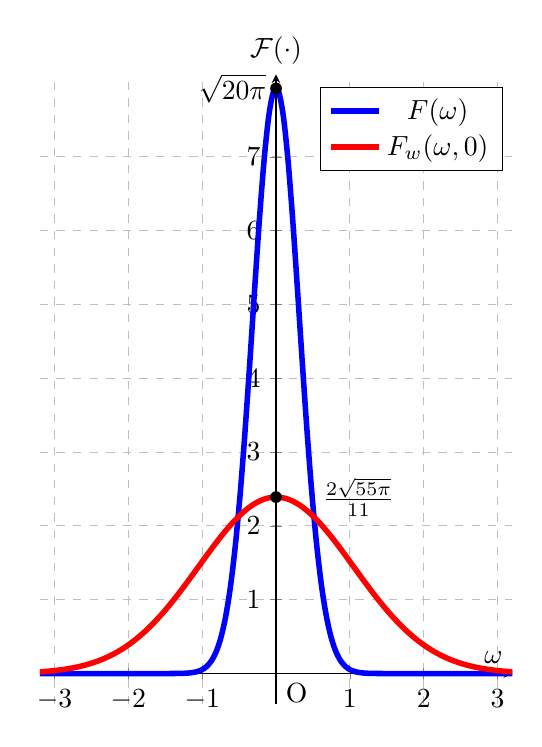
\begin{tikzpicture}
                    \begin{axis}[
                        axis lines = middle,
                        xlabel = {$\omega$},
                        ylabel = {$\mathcal{F}(\cdot)$},
                        ylabel style={at={(rel axis cs:0.5, 1)}, anchor=south},
                        xmin = -3.2, xmax = 3.2,
                        ymin = -0.2, ymax = 7.9,
                        xtick distance = 1,
                        ytick = {1, 2, 3, 4, 5, 6, 7},
                        grid = major,
                        grid style = dashed,
                        scale only axis,
                        width = 6cm,
                        height = 8cm,
                        axis equal,
                    ]
                    \addplot[domain=-3.2:3.2, samples=100, smooth, line width=2pt, blue] {sqrt(20 * pi) * exp(-5 * x^2)};
                    \addlegendentry{$F(\omega)$}
                    \addplot[domain=-3.2:3.2, samples=100, smooth, line width=2pt, red] {sqrt(20 / 11 * pi) * exp(-5 / 11 * x^2)};
                    \addlegendentry{$F_w(\omega, 0)$}
                    \node at (axis cs:0, 0) [anchor=north west] {O};
                    \node[circle, fill, inner sep=1.5pt] at (axis cs:0, 7.927) {};
                    \node at (axis cs:0, 7.927) [anchor=east] {$\sqrt{20\pi}$};
                    \node[circle, fill, inner sep=1.5pt] at (axis cs:0, 2.390) {};
                    \node at (axis cs:0.5, 2.390) [anchor=west] {$\frac{2\sqrt{55\pi}}{11}$};
                    \end{axis}
                \end{tikzpicture}
                \caption{频谱图像对比}
                \label{fig:chap2-part6-exercise1-solution}
            \end{figure}
            可以看出,这两个频率谱在 $\omega = 0$ 处均有峰值,但 $F(\omega)$ 的峰值更高,
            为 $F_w(\omega, 0)$ 的 $\sqrt{11}$ 倍。同时,$F_w(\omega, 0)$ 比 $F(\omega)$ 更加
            “平缓”,即 $F_w(\omega, 0)$ 的峰值附近的值相对于峰值更小。
    \end{enumerate}
\end{solution}

\subsubsection{采样与混叠}

\begin{definition}[混叠]
    当采样周期变大时,频谱的周期会变小。此时,离散信号的谱会发生相互重叠的现象。
    这种现象称为\bd{混叠}。
\end{definition}

\begin{example}
    如图 \ref{fig:aliasing-example-1} 和 \ref{fig:aliasing-example-2} 所示,
    当采样频率 $T_s$ 变大时,信号 $F_s(\omega)$ 会发生混叠。
    \begin{figure}[H]
        \centering
        \begin{subfigure}{0.45\textwidth}
            \centering
            \includegraphics[width=\textwidth]{chap2/img/aliasing-example-1.png}
            \caption{采样频率 $T_s$ 较小}
            \label{fig:aliasing-example-1}
        \end{subfigure}
        \hfill
        \begin{subfigure}{0.45\textwidth}
            \centering
            \includegraphics[width=\textwidth]{chap2/img/aliasing-example-2.png}
            \caption{采样频率 $T_s$ 较大}
            \label{fig:aliasing-example-2}
        \end{subfigure}
        \caption{混叠现象}
    \end{figure}
\end{example}

\begin{example}
    设如图 \ref{fig:aliasing-example-3} 所示的模拟音频信号
    高频截止频率为 $f_M = 5\;\mathrm{kHz}$,采样频率为 $6\;\mathrm{kHz}$。
    问:抽样后信号频谱与原信号频谱在 $2\;\mathrm{kHz}$ 处有什么差异?
    \begin{figure}[H]
        \centering
        \includegraphics[width=0.8\textwidth]{chap2/img/aliasing-example-3.png}
        \caption{模拟音频信号的频谱}
        \label{fig:aliasing-example-3}
    \end{figure}
\end{example}

\begin{solution}
    采样后的频谱相当于原信号的频谱以 $6\;\mathrm{kHz}$ 为周期进行叠加。
    在 $2\;\mathrm{kHz}$ 处的频谱为原 $2\;\mathrm{kHz}$ 处的频谱
    与 $4\;\mathrm{kHz}$ 处的频谱的叠加。
    % TODO:大小会变成原来的 1/6000 倍吗?
    画出采样后的频谱如图 \ref{fig:aliasing-example-4} 所示。
    \begin{figure}[H]
        \centering
        \includegraphics[width=0.8\textwidth]{chap2/img/aliasing-example-4.png}
        \caption{抽样后信号的频谱}
        \label{fig:aliasing-example-4}
    \end{figure}
\end{solution}

\begin{remark}
    思考:混叠对音频质量会产生什么影响?
    % TODO:问混叠对音频质量会产生什么影响?
\end{remark}

\begin{remark}
    思考:如何防止混叠?
    % TODO:问如何防止混叠?
\end{remark}

\subsubsection{采样定理}

要想使采样后的信号样本能完全代表原来的信号,
就意味着要能够从 $X_p(\mathi \omega)$中不失真地分离出 $X(\mathi \omega)$。
这就要求 $X(\mathi \omega)$ 在周期性延拓时不能发生频谱的混叠。
为此必须要求:
\begin{enumerate}
    \item $x(t)$ 必须是带限的,最高频率为 $\omega_M$。
    \item 采样间隔(周期)不是任意的,必须保证采样频率 $\omega_s \ge 2\omega_M$。
\end{enumerate}
在满足上述要求时,可以通过理想低通滤波器从 $X_p(\mathi \omega)$ 中
不失真地分离出 $X(\mathi \omega)$。

\begin{theorem}[Nyquist 采样定理]
    设 $x(t)$ 是带限信号,其最高频率为 $\omega_M$。
    如果以 $\omega_s > 2\omega_M$ 的频率进行采样,则 $x(t)$ 可以唯一地
    由其样本 $x(nT_s)$ 决定,其中 $T_s = 2\pi/\omega_s$。
\end{theorem}

\begin{example}[采样定理的图示]
    如图 \ref{fig:sampling-theorem} 所示为两种不同的采样频率 $\omega_s$ 下的采样效果。
    其中 $\omega_c$ 为过渡带的截止频率。
    \begin{itemize}
        \item 当 $\omega_s > 2\omega_M$ 时,采样后的频谱不会发生混叠,过渡带将两个周期的频谱分开。
        \item 当 $\omega_s < 2\omega_M$ 时,采样后的频谱会发生混叠,过渡带处两个周期的频谱混合在一起。
    \end{itemize}
    \begin{figure}[H]
        \centering
        \includegraphics[width=0.45\textwidth]{chap2/img/sampling-theorem.png}
        \caption{采样定理的图示}
        \label{fig:sampling-theorem}
    \end{figure}
\end{example}

\begin{example}
    在工程实际应用中,理想滤波器是不可能实现的。而非理想滤波器一定有过渡带,
    也就是如图 \ref{fig:real-sampling-theorem} 所示中
    的 $\omega_c \in (\omega_M, \omega_s - \omega_M)$。
    因此,实际采样时,$\omega_s$ 必须大于 $2\omega_M$。
    \begin{figure}[H]
        \centering
        \begin{subfigure}{0.45\textwidth}
            \centering
            \includegraphics[width=\textwidth]{chap2/img/real-sampling-theorem.png}
            \caption{实际情况下的采样定理的图示}
            \label{fig:real-sampling-theorem}
        \end{subfigure}
        \hfill
        \begin{subfigure}{0.45\textwidth}
            \centering
            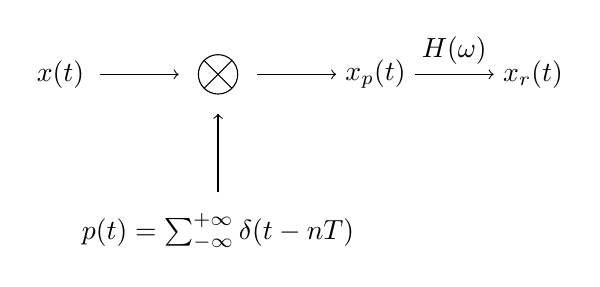
\begin{tikzpicture}
                \draw (0,0) circle (0.25);
            
                \draw (-0.177,-0.177) -- (0.177,0.177);
                \draw (0.177,-0.177) -- (-0.177,0.177);
            
                \draw[->] (-1.5,0) -- (-0.5,0);
                \draw[->] (0.5,0) -- (1.5,0);
                \draw[->] (0,-1.5) -- (0,-0.5);
                \draw[->] (2.5,0) -- (3.5,0) node[midway,above] {$H(\mathi\omega)$};
            
                \node at (-2,0) {$x(t)$};
                \node at (2,0) {$x_p(t)$};
                \node at (0,-2) {$p(t) = \sum_{-\infty}^{+\infty}\delta(t - nT)$};
                \node at (4,0) {$x_r(t)$};
            \end{tikzpicture}
            \caption{实际情况下的采样定理的数学模型}
            \label{fig:real-sampling-theorem-math-model}
        \end{subfigure}
        \caption{实际情况下的采样定理}
    \end{figure}
\end{example}

\begin{property}[三角脉冲的傅里叶变换]
    设 $f(t)$ 为 $[T_0, T_0]$ 上的三角脉冲信号,如图 \ref{fig:triangular-rectangular-1} 所示。
    \begin{figure}[H]
        \centering
        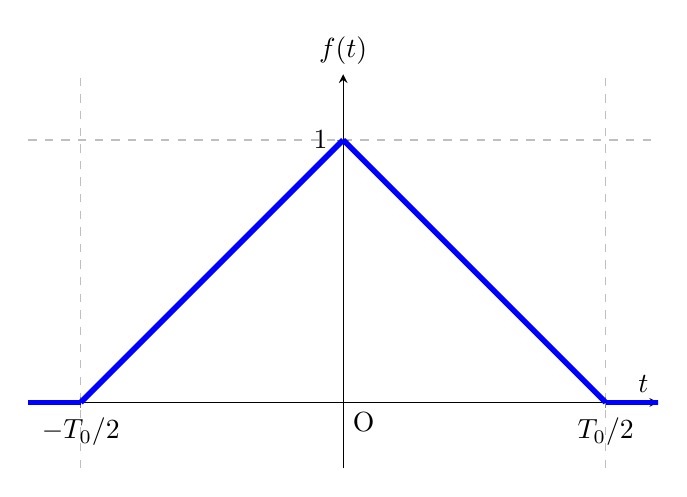
\begin{tikzpicture}
            \begin{axis}[
                axis lines = middle,
                xlabel = {$t$},
                ylabel = {$f(t)$},
                ylabel style={at={(rel axis cs:0.5, 1)}, anchor=south},
                xmin = -1.2, xmax = 1.2,
                ymin = -0.2, ymax = 1.2,
                xtick = {-1, 0, 1},
                xticklabels = {$-T_0/2$, $ $, $T_0/2$},
                ytick distance = 1,
                grid = major,
                grid style = dashed,
                scale only axis,
                width = 8cm,
                height = 5cm,
                axis equal,
            ]
            \addplot[domain=-1.2:-1, samples=100, smooth, line width=2pt, blue] {0};
            \addplot[domain=-1:0, samples=100, smooth, line width=2pt, blue] {x + 1};
            \addplot[domain=0:1, samples=100, smooth, line width=2pt, blue] {-x + 1};
            \addplot[domain=1:1.2, samples=100, smooth, line width=2pt, blue] {0};
            \node at (axis cs:0, 0) [anchor=north west] {O};
            \end{axis}
        \end{tikzpicture}
        \caption{三角信号 $f(t)$}
        \label{fig:triangular-rectangular-1}
    \end{figure}
    则其傅里叶变换为
    \begin{align*}
        H(\mathi\omega) = T_0\cdot \sa^2\left(\frac{\omega T_0}{2}\right).
    \end{align*}
\end{property}

\begin{proof}
    三角脉冲可以表示为两个矩形脉冲的卷积。记 $g(t)$ 为 $[-T_0/2, T_0/2]$ 上的矩形脉冲信号,
    脉宽 $\tau = T_0$,脉高 $E = \sqrt{1/T_0}$,如图 \ref{fig:triangular-rectangular-2} 所示。
    \begin{figure}[H]
        \centering
        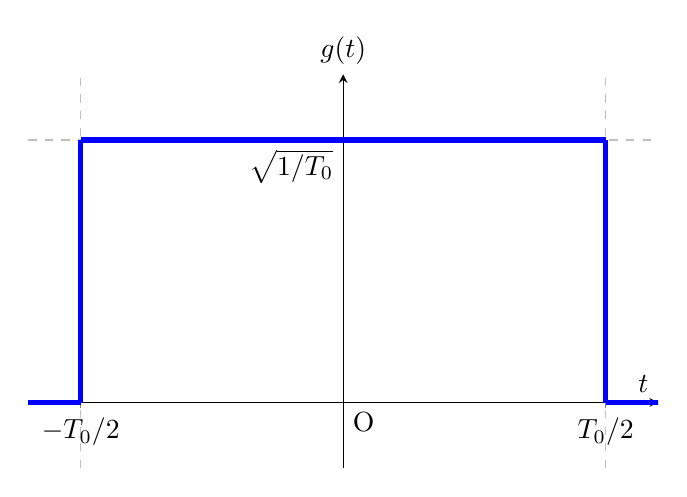
\begin{tikzpicture}
            \begin{axis}[
                axis lines = middle,
                xlabel = {$t$},
                ylabel = {$g(t)$},
                ylabel style={at={(rel axis cs:0.5, 1)}, anchor=south},
                xmin = -1.2, xmax = 1.2,
                ymin = -0.2, ymax = 1.2,
                xtick = {-1, 0, 1},
                xticklabels = {$-T_0/2$, $ $, $T_0/2$},
                ytick = {0, 1},
                yticklabels = {$ $, $ $},
                grid = major,
                grid style = dashed,
                scale only axis,
                width = 8cm,
                height = 5cm,
                axis equal,
            ]
            \addplot[domain=-1.2:-1, samples=100, smooth, line width=2pt, blue] {0};
            \addplot[smooth, line width=2pt, blue] coordinates {(-1, 0) (-1, 1)};
            \addplot[domain=-1:0, samples=100, smooth, line width=2pt, blue] {1};
            \addplot[domain=0:1, samples=100, smooth, line width=2pt, blue] {1};
            \addplot[smooth, line width=2pt, blue] coordinates {(1, 1) (1, 0)};
            \addplot[domain=1:1.2, samples=100, smooth, line width=2pt, blue] {0};
            \node at (axis cs:0, 0) [anchor=north west] {O};
            \node at (axis cs:0, 1) [anchor=north east] {$\sqrt{1/T_0}$};
            \end{axis}
        \end{tikzpicture}
        \caption{矩形脉冲信号 $g(t)$}
        \label{fig:triangular-rectangular-2}
    \end{figure}
    因此,$f(t) = g(t) * g(t)$。由卷积定理知
    \begin{align*}
        H(\mathi\omega) & = G(\mathi\omega) \cdot G(\mathi\omega) \\
        & = \left(E\tau\sa\left(\frac{\omega\tau}{2}\right)\right)^2 \\
        & = T_0\cdot \sa^2\left(\frac{\omega T_0}{2}\right).
    \end{align*}
\end{proof}

\subsubsection{采样定理的方法论思考}

% TODO:PPT 的逻辑

关键科学问题

\bd{局部}如何选择,才能全面体现\bd{整体}的变化规律?

信号处理:抽样定理对抽样频率的约束。

\begin{figure}[H]
    \begin{tikzpicture}
        % Nodes
        \node at (3,2) [text width=12cm] (title) {多媒体计算机智能处理与应用};
        \node at (-2,0)[text width=5cm] (analog) {模拟(连续)世界};
        \node at (4,0)[text width=5cm] (digital) {数字(离散)世界};
        
        % Arrows
        \draw[->] (-1.5,0) -- (1.5,0)
        node[midway, above] {抽样} 
        node[midway, below] {桥梁};
        
        \draw[->] (3,0.5) -- (0,1.5)
        node[midway, right] {提取特征、改变特征};
        
    \end{tikzpicture}
\end{figure}

\begin{example}
    设模拟音频信号高频截止频率为 $10\;\mathrm{kHz}$。若抽样频率为 $16\;\mathrm{kHz}$,
    则抽样后信号频谱与原信号频谱在 $12\;\mathrm{kHz}$ 处有什么差异?
\end{example}

\begin{example}
    模拟信号(实信号)频率在 $850\;\mathrm{kHz}$ 到 $900\;\mathrm{kHz}$。
    若采样频率为 $200\;\mathrm{kHz}$,则采样后信号频谱在 $20\;\mathrm{kHz}$ 处
    与原信号有什么差异?
    (要求:文字说明幅度的变化;如果有混叠发生,请说明混叠对应的原频谱)
\end{example}

% TODO:问这两题答案
